\documentclass[11pt,letterpaper]{article}
\usepackage[margin=1in]{geometry}
\usepackage{amsmath,amssymb,booktabs,longtable,tabularx,array,xcolor,hyperref,fancyhdr,microtype,tikz}
\hypersetup{colorlinks=true,linkcolor=blue!45!black,citecolor=blue!45!black,urlcolor=blue!50!black,pdftitle={CRGC Master Whitepaper v0.2},pdfauthor={AI-assisted research synthesis prepared for Justin Candler}}
\setlength{\parindent}{0pt}\setlength{\parskip}{6pt}\setlength{\emergencystretch}{3em}
\newcolumntype{P}[1]{>{\raggedright\arraybackslash}p{#1}}
\newcommand{\E}{\mathbb E}\newcommand{\R}{\mathbb R}\newcommand{\CRGC}{\operatorname{CRGC}}
\newcommand{\status}[1]{\textbf{Evidence status:} #1}
\pagestyle{fancy}\fancyhf{}\fancyhead[L]{\small CRGC master whitepaper / v0.2}\fancyhead[R]{\small 24 November 2026}\fancyfoot[C]{\thepage}\setlength{\headheight}{14pt}
\begin{document}
\hypersetup{pageanchor=false}\begin{titlepage}
{\large CONFIDENTIAL RESEARCH DISCUSSION DRAFT\par}\vspace{1.3cm}
{\Huge\bfseries Computationally Recoverable\\[5pt] Grid Capability\par}\vspace{0.7cm}
{\LARGE A rigorous framework for testing the value of better computation on fixed electrical infrastructure\par}\vspace{0.7cm}
{\Large Master whitepaper v0.2\par}
24 November 2026 \quad | \quad Evidence cutoff: 24 November 2026
\vspace{0.8cm}

Prepared for Justin Candler\\AI-assisted research synthesis and preliminary computational study
\vspace{0.7cm}

\textbf{Central finding.} Better decisions can improve useful electrical service on unchanged equipment. The magnitude is an empirical question about a specified baseline, information set, deadline, and reliability contract. Neither a complexity separation nor an optimization gap establishes an energy resource.

\textbf{Results in this edition.} A three-bus AC-OPF experiment finds no material benefit from nine additional starting points. A synthetic BESS experiment finds improved service against a limited threshold policy, but that advantage disappears against a simple forecast-aware threshold policy. An exact-arithmetic certificate demonstration rejects four altered witnesses. These are preliminary model results, not field savings.

\textbf{VP/VNP assessment.} The November 2026 releases claim superpolynomial arithmetic-circuit lower bounds and include formal proof artifacts. The supplied six-pass review and external machine-check report strengthen specific verification evidence, while leaving independent mathematical review obligations. No reduction or algorithm in this edition connects the separation to an AC-OPF or SCUC speedup.

\vfill
\textbf{Provenance boundary.} The original Billion-Dollar Napkin is preserved byte-for-byte. The referenced chat's v0.1 download files were unavailable; its truncated inline source is preserved separately. This edition is a new standalone synthesis, not a certified line-by-line revision of an intact v0.1. Local Library routes and selected Drive research were searched; the complete native Library and its Atlas were not verified. No original research files were edited or moved.
\end{titlepage}\hypersetup{pageanchor=true}\pagenumbering{roman}
\begin{abstract}
Computationally recoverable grid capability (CRGC) denotes a measured improvement in electrical service or resource cost attributable to a computational intervention under an explicit operational contract. We separate improvements in physical dispatch, feasible-set information, policy design, verification, and hardware. This distinction prevents congestion payments, electrical losses, reserve requirements, unserved energy, and capacity accreditation from being combined into a fictitious additive resource. A critical review connects arithmetic complexity, AC relaxations, unit commitment, model predictive control, formal verification, and large-load storage without assuming a new universal solver. We reconstruct the Billion-Dollar Napkin's arithmetic and identify the unsupported causal assumptions behind its national totals. We report reproducible experiments, including a stronger comparator that eliminates the apparent optimization-specific benefit in constructed battery scenarios. The resulting research program is falsifiable: benefit must survive strong baselines, independent feasibility checks, equal information and resource budgets, uncertainty, adverse operating conditions, and a separately defined economic accounting boundary. The paper provides a bounded literature and source audit, explicit upper bounds, a claim-evidence map, and a staged evaluation protocol. It does not establish national recoverable TWh, firm MW, commercial savings, or a production-ready controller.
\end{abstract}
\tableofcontents\newpage\pagenumbering{arabic}
\section{The proposition and the decision it should support}
\label{sec:proposition}
The useful proposition is narrower than the idea that software creates generation: on a given network, a better operational decision may deliver the same service at lower real resource cost, or more valuable service at the same acceptable risk. Better dispatch can reduce avoidable congestion and losses; a better commitment can avoid expensive starts; a better controller can reduce tracking error; stronger evidence can permit an otherwise defensible action to be approved. None of these mechanisms is guaranteed to be positive on a particular system.

CRGC is an attribution and measurement framework, not a newly proved complexity class or a claim that previous optimization research overlooked computation. Its potentially distinctive contribution is a common accounting contract across grid operations, power electronics, and computational loads: identify the action changed, preserve the physical and informational boundary, measure service and cost separately, and expose the evidence needed for operational acceptance.

For a development or investment decision, three questions come first. Is there an observed operational bottleneck that computation can affect? Does the proposed intervention outperform a credible current alternative on the same task? Does the gain survive the cost of implementing, validating, maintaining, and operating it? A positive answer to a mathematical question alone does not answer any of these.

\subsection{What this edition changes}
The Napkin is retained as an originating hypothesis, not as an established resource assessment. Its arithmetic is reconstructed in Section~\ref{sec:napkin}; its national recovery percentages are excluded from admitted findings. The VP/VNP claims are moved to the front because they motivate interest in AI-assisted mathematical discovery, but their mathematical scope is stated before discussing transfer. Internal research contributes definitions and questions; independent primary literature supplies external observations. Preliminary tests report null results and comparator sensitivity instead of selecting only favorable outcomes.

The supplied \texttt{VP\_VNP\_Review} folder arrived during this study. Its Edition~3 handoff and all six pass records were read. Three accompanying Python checks were rerun from copies. The folder's prompt for another proof pass is treated as documentary content, not an instruction to modify that review or to substitute its agenda for this paper.

\subsection{Claim vocabulary}
Throughout this paper, \emph{measured} means obtained in the attached local computation unless a field dataset is explicitly named. \emph{Reported} means a source's observation or claimed theorem, not independently reproduced here. \emph{Derived} means a transparent calculation or conditional mathematical argument in this paper. \emph{Projected} means a future scenario. \emph{Proposed} means an unrun mechanism or experiment. These categories are not interchangeable.

An internal analysis can accurately summarize an external source, but its reuse does not add an independent evidence group. A Drive copy and a local copy of one paper are one lineage. A theorem author, its repository, and its CI logs provide distinct artifacts within one publisher lineage; they are not three independent mathematical endorsements.

\section{November 2026 VP/VNP claims: precise scope and evidence}
\label{sec:vp}
\subsection{What is being separated}
An arithmetic circuit is a finite directed computation using field constants, variables, additions, and multiplications; subtraction is expressible using the constant $-1$. Its output is a \emph{formal polynomial}. It can reuse intermediate results, exploit cancellation, and vary with input dimension. Arithmetic gate count is not the bit complexity of a floating-point optimizer.

VP consists of polynomial families with polynomially bounded numbers of variables, degrees, and arithmetic-circuit sizes. VNP permits a sum over polynomially many auxiliary Boolean coordinates of a VP family. The exponential number of summands does not by itself prove hardness: many large sums have compact expressions. The separation claims address every permitted circuit, not merely an enumeration algorithm.

The Anthropic statement file defines circuit size to include variable and constant gates. For a generic $m\times m$ matrix,
\[
 \operatorname{PERM}_m(X)=\sum_{\sigma\in S_m}\prod_{i=1}^m X_{i,\sigma(i)},\qquad
 \operatorname{HC}_m(X)=\sum_{\substack{\sigma\in S_m\\\sigma\text{ one cycle}}}\prod_{i=1}^m X_{i,\sigma(i)}.
\]
The claimed exact theorem has the quantifier order
\begin{equation}
 \exists c>0\;\forall p\;\exists m_0(p)\;\forall F:\operatorname{char}F=p\;
 \forall m\ge m_0(p),\quad
 \operatorname{size}(\operatorname{HC}_m)>m^{c(\log_2m)^{1/3}} .
 \label{eq:vp}
\end{equation}
The permanent has the same claim when $p\ne2$. Characteristic two is excluded for the permanent because it equals the determinant there. The threshold is uniform over fields of a given characteristic; the positive constant is outside that quantifier. The claimed consequence is VP strictly contained in VNP over every field.\cite{anthropicstatement}

The separate approximate statement concerns circuits over formal Laurent series whose nonpositive coefficients match the target polynomial: negative coefficients vanish and the constant coefficient is the target. This is border complexity, not a numerical guarantee for a fixed engineering error tolerance. It supplies no bound on floating-point conditioning, finite precision, or acceptable OPF constraint residuals.\cite{anthropicstatement}

\subsection{What the two primary releases report}
Claude/Anthropic's 70-page paper uses tensor restrictions and spectral points to obtain realizable distance functions, called prices. A crossing-wires identity constrains their geometry. The proof splits into a flat branch, using Euclidean configurations and balanced tensor cuts, and a contracting branch, using laws, trees, and cuts of weighted computations. A hypothetical small circuit leads to an accelerating evaluator contradicted through diagonalization. This is a lower-bound argument, not an executable optimization recipe. The paper's Theorems~1.1 and~1.4 state exact and border results; Appendix~Q discusses correspondence qualifications. Remark~N.6's determinantal consequence is not part of the release's completed formal proof coverage.\cite{anthropic}

OpenAI's distinct November~23 manuscript states a border lower bound $\exp(\Omega((\log n)^{5/4}))$ for an explicit weighted accepting-path polynomial family over every field. Its construction uses an $n^{1000}$ clock for accepting paths of a universal machine and transfers the bound to HC and, outside characteristic two, the permanent. The proof describes Euclidean tensor pricing, boundary slicing, residues, and replay within wire budgets. Its repository also links a Lean proof of exact VP--VNP separation. That link alone does not establish that every border theorem in the PDF has been replayed or formalized here.\cite{openai}

The two papers should be cited separately. Agreement on a headline does not independently validate either proof. This study inspected the primary statements and proof architecture; it did not reconstruct either full proof or replay either complete formal build.

\subsection{Verification evidence, with separate scopes}
The Anthropic README reports AI authorship of both paper and proof and explicitly states that no human mathematician had checked the proof. The released workflow includes a Lean build, axiom inspection, Comparator, and another kernel checker. The intentionally incomplete \texttt{Challenge.lean} template must not be mistaken for an admitted theorem in the submitted solution. A reliable audit must inspect the dependency closure of the final theorem.\cite{anthropicrepo}

Carlos Toledo's independent public audit, in its build through 03:15 UTC on November~24, reports 18 of 23 registered rows passed and a CERTIFIED verdict under its specified machine-check rule. It reports multiple kernels, a second machine, blind statement bridges, and mutation controls. It also explicitly disclaims human mathematical review and says Claude models perform much of the checking. Thus its operational independence does not imply model-family independence. Its remaining work includes a determinantal consequence and a readable account. These are the audit's reported results, not checks rerun in this CRGC study.\cite{toledo}

The user-supplied review pins publisher commit
\texttt{11b6c7e3c927df2658f513b6b68ea7f8929c62c5}. Its PDF hash is recorded in the companion source inventory. This study recomputed that hash and matched its \texttt{Statement.lean} to the separately downloaded statement. The Hexagon PDF downloaded earlier has a different byte hash; these editions are retained as distinct artifacts rather than silently merged. The supplied review records publisher CI success and focused Lean checks, while explicitly leaving full local replay open.\cite{internalvp}

\subsection{What the six-pass internal review adds}
The review traces the entry of arbitrary circuits into both branches, rather than assuming that a bound for a restricted circuit family suffices. Its flat-branch analysis identifies the cost of summing pieces across different balanced cuts; it rejects the shortcut of imposing one common cut on the whole sum. Its contracting analysis distinguishes a bound on each accepting run from deterministic evaluation of the sum over all runs. An exponentially large sum remains possible.

Two prose qualifications are especially useful. First, a zero-weight accepting source run can disappear in the pointer interpreter while preserving the weighted value. Second, the cutter can omit an active-wire assignment when the corresponding product has a zero factor. Neither observation alone refutes the scalar identity consumed downstream. The review also distinguishes universal halting from a deadline for every rejecting run. These are examples of why an operational contract must name the observable being preserved: value, multiplicity, termination, and runtime are different properties.

This study reran the review's exact algebra examples, four finite pointer-trace cases, and 15 cut-resource cases. The assertions passed. The four trace cases retain values $0,-1,2,0$, including zero-weight elimination and cancellation. These finite checks do not establish the general simulation theorem. The review leaves the geometric alternative D.2, foundational tower and piece identities, and a complete independent Lean replay as open obligations. Its recommended next derivation was not performed here.\cite{internalvp}

\subsection{Why this does not solve AC-OPF or SCUC}
The inference that VP differs from VNP and therefore grid optimization becomes easy is a non sequitur. A lower bound says certain polynomial families lack small circuits in a specified model. It neither supplies a faster grid algorithm nor identifies the practical distribution of hard grid cases. AC power-balance equations can be evaluated efficiently even when finding a feasible or optimal operating point is difficult. Evaluating those equations is not the same task as computing the permanent.

SCUC is usually formulated as a mixed-integer optimization problem with temporal and security constraints. A connection to an arithmetic-circuit family would require an explicit reduction with preserved size, coefficient precision, approximation target, and objective meaning. None is supplied in the reviewed artifacts. Boolean P versus NP remains separate. A polynomial-time linear optimization algorithm should not be described as membership of the grid optimization problem in VP: these refer to different computational objects.

Even quantitative lower bounds can be operationally uninformative at practical dimensions. Toledo's reading gives $c=1/1600^2$ for the Anthropic proof and no explicit $m_0$.\cite{toledo} Conditional on that constant, the displayed exponent exceeds two only if
\[
 \log_2m>(2\cdot1600^2)^3
   =134{,}217{,}728{,}000{,}000{,}000{,}000.
\]
This algebraic comparison is not a verified onset threshold for the theorem and is not a runtime estimate.

\subsection{Testable transfer mechanisms}
\begin{longtable}{P{.19\linewidth}P{.37\linewidth}P{.35\linewidth}}
\toprule Mechanism & Concrete experiment & Falsifier or limitation\\\midrule\endhead
Formal discovery workflow & AI proposes inequalities or algebraic rewrites; a separate checker validates them. Compare established cuts and equal tuning budgets. & No improvement after checking overhead, rejected certificates, or gains lost against established cuts.\\
Structure-guided decomposition & Use graph separators, chordal structure, or low-dimensional coupling to select subproblems. & Construction costs exceed savings or physical coupling prevents separation. This is inspired research, not an extracted VP/VNP algorithm.\\
Proof-carrying decisions & Export a dual witness, interval feasibility enclosure, or checkable discrete proof artifact. Measure verification cost. & The encoding omits a physical constraint or checking misses the deadline.\\
Compiler specialization & Generate fixed-structure control code with bounded memory and arithmetic. & Timing, stability, or numerical margin fails outside nominal parameters.\\
Hardness-aware fallback & Detect a class admitting a bounded method and fall back otherwise. & Detection is unreliable or costs as much as solving. Asymptotic hardness alone supplies no detector.\\
\bottomrule
\end{longtable}
None of these mechanisms requires the VP/VNP theorem to be accepted before it can be tested. That independence is scientifically useful: the grid research program can survive a revision of the mathematical claim.

\section{A precise operational definition}
\label{sec:definition}
Let $\omega$ denote a chronological realization of demand, weather, outages, prices, and available observations. Let $\mathcal I_t$ be the information actually available at decision time $t$. A policy $\pi$ maps the observation history to controls; it must be nonanticipative. Specify a contract
\[
 \mathcal K=(N,H,\mathcal I,B,d,\varepsilon,\mathcal V,\mathcal F),
\]
where $N$ is the network and equipment, $H$ the horizon and time resolution, $B$ the compute budget including preprocessing and checking, $d$ the action deadline, $\varepsilon$ the accepted risk/tolerances, $\mathcal V$ the validation model, and $\mathcal F$ the fallback policy. Budgets may include energy, capital cost, memory, and operator effort as well as processor time.

Define a vector of outcomes
\[
 Q(\pi,\omega)=
 \big(E_{\rm served},E_{\rm loss},E_{\rm curtailed},
 C_{\rm resource},R_{\rm adequacy},R_{\rm dynamic},
 T_{\rm latency},E_{\rm compute}\big).
\]
Units and preferences differ across coordinates. For a named service metric $q$ whose larger value is preferable,
\begin{equation}
 \CRGC_q(\pi_1;\pi_0\mid\mathcal K)
  =\E_{\omega\sim P}\!\left[q(\pi_1,\omega)-q(\pi_0,\omega)\right],
 \label{eq:crgc}
\end{equation}
subject to both policies meeting $\mathcal K$. A reduction in resource cost instead uses $C(\pi_0)-C(\pi_1)$. Negative values must be retained. A policy that fails the safety contract does not obtain a favorable service score by ignoring its violations.

\subsection{Five interventions that must be separated}
\textbf{Algorithm intervention:} change the numerical method while holding formulation, data, information, hardware, and deadlines fixed. This is the narrowest computational attribution.

\textbf{Policy intervention:} change the objective, planning horizon, reserve policy, or decision rule. It can be valuable, but a gain against a weak policy does not establish a solver advance. The BESS experiment in Section~\ref{sec:results} illustrates this distinction.

\textbf{Information intervention:} improve forecasts, telemetry, state estimation, or line ratings. Changing an assumed limit can alter the feasible set even if the optimizer is unchanged. Attribute the gain to information and operational authorization, with computation as an enabling component where demonstrated.

\textbf{Assurance intervention:} produce stronger evidence that a proposed action is admissible. A certificate can remove uncertainty about a model without changing dispatch. Record the decision that assurance changes before assigning economic value.

\textbf{Hardware intervention:} add storage, conductors, inverter capacity, sensing, or compute hardware. Record capital and physical changes separately. A faster processor is a compute investment; it is not a free algorithmic improvement.

For two interventions $A$ and $I$, run a $2\times2$ comparison and report the interaction
\[
 \Delta_{AI}=Q_{11}-Q_{10}-Q_{01}+Q_{00}.
\]
Without all cells, allocating a joint gain between information and algorithm is convention-dependent. Do not add each stand-alone gain to the joint gain.

\subsection{Feasibility, optimality, and usefulness}
An optimizer's success flag is not an independent feasibility certificate. Reconstruct power balance and branch flows separately, document units and tolerances, test both ends of thermal constraints, and include all required contingencies. A lower-cost infeasible point is not a valid improvement.

For a minimization problem, a validated feasible objective $U$ and a valid lower bound $L$ imply
\begin{equation}
 0\le U-C^\star\le U-L.
 \label{eq:gap}
\end{equation}
This is an upper bound on possible improvement within that same model. Tightening $L$ can reduce the certificate gap while leaving $U$ and the physical dispatch unchanged. If the candidate improves the feasible objective from $U_0$ to $U_1$, the observed model improvement is $U_0-U_1$, not the initial gap.

A model's optimum is not necessarily the best real-world action: missing dynamics, parameter error, imperfect forecasts, and unpriced consequences can reverse the ordering. Validation therefore needs an operationally credible evaluation model and, later, a controlled deployment design.

\section{Literature synthesis and novelty boundary}
\label{sec:literature}
\subsection{Grid optimization is already a substantial research program}
ARPA-E's Grid Optimization Competition supplies a precedent for comparing algorithms on common data and compute resources. PNNL's 2024 supporting report describes three challenge generations spanning security-constrained AC optimization, devices and switching, and multiperiod operations. It reports \$9.24 million in prizes and nearly 30 million CPU-hours. The frequently repeated claim that a one-percent efficiency improvement could save a billion dollars is a program motivation, not an observed realized saving. Competition performance, deployment, and annual economic impact must be assessed separately.\cite{go}

PGLib-OPF provides standardized AC-OPF formulations and cases, including stressed variants. It is a benchmark library, not a distribution of a specific utility's current operations. A result on a small case is useful for exercising a method but supplies little evidence about national value.\cite{pglib} PGLib-UC likewise makes unit-commitment instances reproducible; its documented core is a global demand-and-reserve formulation. It must not be relabeled a complete network- and contingency-constrained SCUC benchmark.\cite{pglibuc}

\subsection{AC relaxations: known routes to bounds, conditional exactness}
Low's two-part review establishes the relationship among common OPF relaxations and the conditions under which a relaxation can recover a feasible optimum. Topology, operating bounds, objectives, and other assumptions matter; radial topology alone is not a universal exactness guarantee.\cite{low1,low2} Sparse moment relaxations pursue stronger bounds while exploiting network structure; selective higher-order constraints are existing methodology, not a novel consequence of VP/VNP.\cite{moment}

These methods create two distinct research opportunities. A tighter lower bound can quantify how little cost improvement remains possible. A method that recovers a better feasible point can change an actual decision. Report both trajectories, including total solve time. A relaxation that returns a lower objective but no feasible recovery has supplied evidence about a bound, not a usable dispatch.

Worst-case AC-feasibility hardness results demonstrate the limits of expecting universal tractability in sufficiently general formulations.\cite{hardness} They do not establish that operational instances are uniformly hard, that every heuristic is unreliable, or that a proposed method will outperform current practice. The gap between structural special cases and general hardness is where benchmark design matters.

\subsection{Unit commitment and operational simulation}
Unit commitment combines binary commitment decisions with starts, minimum up/down times, ramps, costs, and reserve requirements. Network and contingency constraints add further structure. Knueven, Ostrowski, and Watson show why comparing formulations and combining strong components is a serious baseline requirement.\cite{uc} A new method should face contemporary formulations and solver settings rather than an intentionally weak mixed-integer model.

Recent relax-and-round work with sub-hourly mechanical and ramp constraints is directly relevant to faster feasible schedules.\cite{round} Its results should be read against the exact instances, tolerances, and hardware in the paper. The existence of a fast heuristic does not establish its optimality or its benefit on MISO's production system. Likewise, a mixed-integer relative gap can be a stopping criterion without representing avoidable electrical energy.

Lara and colleagues' operations-model experiment design emphasizes the timing and coupling of decision models.\cite{experiment} This supports chronological evaluation with forecasts issued at realistic times and commitments carried across intervals. Solving every hour with hindsight can create infeasible schedules or an artificial value of perfect information.

\subsection{MPC and implementation constraints}
Model predictive control repeatedly optimizes over a horizon and applies only the next action. Its usefulness depends on the dynamics, constraints, estimator, horizon, terminal treatment, timing, and fallback. An hourly battery scheduling LP is not evidence of microsecond inverter control.

Jeong and collaborators report hardware implementations of long-horizon MPC using FPGA architectures, including ADMM and regionless explicit formulations.\cite{mpc,mpc2} These are implementation precedents with problem-specific measurements. A cited 100\,kHz implementation corresponds to a 10\,$\mu$s sampling period; only part of that period may be available for optimization after measurement, communication, and actuation. Stability and damping analyses are also control-structure dependent.\cite{mpcdamp}

Shoja, Arnstr\"om, and Axehill study parallel domain decomposition for certifying branch-and-bound complexity in multiparametric MILP/MIQP settings.\cite{complexity} A bound on nodes or linear-system iterations is not automatically a wall-clock deadline bound. Processor architecture, memory traffic, numerical behavior, and scheduling must be included in deployment evidence.

\subsection{Formal methods and AI assistance}
Lean-PEP illustrates a concrete separation between numerical certificate discovery, exact finite checking, and an analytic theorem connecting the certificate to the intended algorithmic statement. Its supported models are specific PG/GD settings; it is not a formalization of an entire power grid or a generic nonconvex optimality oracle.\cite{leanpep}

Stechly, Valmeekam, and Kambhampati's study of LLM self-verification concerns specified reasoning and planning tasks and model versions. It supports using an external verifier for those experiments, not a universal claim about every future model.\cite{selfverify} In CRGC, generated constraints, code, and certificates should face independent checks appropriate to their semantics.

Grid-Agent and Grid CoPilot are adjacent work rather than evidence that autonomous grid operation is ready. The former explores LLM-based power-grid analysis and optimization workflows; the latter assists analysis and visualization of long-term production-cost simulations.\cite{gridagent,gridcopilot} Analyst productivity, solver improvement, closed-loop control, and operational authorization are separate endpoints. CRGC's novelty cannot be the generic use of an LLM near a power-system model.

\subsection{Large loads and BESS}
NERC's July 2025 large-load report identifies planning, observability, stability, balancing, and other risks.\cite{nerc} The Library filename labels one copy NREL; its actual publisher is NERC. Source identity was resolved from the contents. A filename should not determine authority.

The June 2026 LBNL update projects 649\,TWh of U.S.\ data-center electricity use in its 2030 reference case, with substantial scenario uncertainty. These are demand projections, not observed 2030 consumption and not a recoverable-loss estimate.\cite{lbnl} A growing load denominator increases the importance of efficient service but does not identify an algorithmic recovery fraction.

Abudyak, Alizadeh, and Sun simulate grid-forming BESS support for data-center loads, including power tracking, reactive support, and islanding.\cite{gfm} Their evidence is simulation evidence; protection coordination, duration, communication, and field validation remain material. Yin and colleagues' work on heterogeneous storage power splitting further illustrates the dependence of results on objective and device characteristics.\cite{split} Neither paper supplies a generic percentage that can be multiplied by all U.S.\ data-center energy.

The internal \emph{Large Loads, IBRs, and the New Grid Bottleneck} frames dependable load service through adequacy, deliverability, stability, and observability. This is useful as a checklist of distinct requirements.\cite{internaldls} The internal Compute/ASCDE/SMR manuscript contains broader thermodynamic and hallucination-entropy hypotheses. No independently supported causal link from those hypotheses to grid recoverability was established; they are excluded from the accepted evidence base.\cite{internalcompute}

\section{Reconstructing the Billion-Dollar Napkin}
\label{sec:napkin}
\status{Arithmetic reconstruction of internal scenario inputs; the inputs and recovery fractions are not admitted as measured recoverable energy.}

The six-page Napkin combines several conceptual pools.\cite{napkin} Table~\ref{tab:napkin} retains its numerical inputs so that the hypothesis remains auditable. PSE denotes its power-systems grouping; PE denotes its power-electronics grouping. The table does not establish that the rows are independent or avoidable.

\begin{table}[ht]
\centering
\begin{tabular}{lrr}
\toprule Napkin pool or calculation & MISO (TWh) & United States (TWh)\\\midrule
Curtailment pool &13.5&25.0\\
Transmission/distribution loss pool &34.5&221.5\\
SCUC/reserve proxy &27.6&177.2\\
PSE subtotal &75.6&423.7\\
PE pool &7.0&45.0\\
Combined pool &82.6&468.7\\
Assumed 10\% of combined pool &8.26&46.87\\
\bottomrule
\end{tabular}
\caption{Reconstruction of the Napkin's scenario arithmetic, not a resource estimate.}\label{tab:napkin}
\end{table}

The monetary expressions in the Napkin use the PSE fraction, not the entire combined pool:
\begin{align*}
 V_{\rm MISO}&=7.56\times10^6\cdot\$53+0.1\cdot\$2.2\times10^9
                  =\$620.68\text{ million},\\
 V_{\rm US}&=42.37\times10^6\cdot\$50+0.1\cdot\$17\times10^9
                  =\$3.8185\text{ billion}.
\end{align*}
These products follow from the stated inputs. They do not establish causal recovery, nonoverlap, marginal value, or implementation cost. The \$17 billion input is not retained as a verified current national total.

\subsection{The accounting problems}
\textbf{Curtailment is not automatically avoidable.} Some curtailed energy is blocked by physical constraints, stability needs, demand timing, or economic choices. Recovering it may require new storage or transmission. A dispatch intervention must identify the actual binding constraint and the safe alternative action.

\textbf{Electrical loss is not automatically inefficiency of computation.} Resistive losses exist even at an optimum. A different dispatch can reduce some losses while increasing fuel cost or affecting security. Transmission, distribution, and converter-loss boundaries may overlap. A measured reduction needs metered or validated flow accounting at a named boundary.

\textbf{Reserve is not an energy-loss pool.} A reserve requirement represents capability held available, with opportunity cost and reliability purpose. Multiplying load by a reserve percentage does not turn that requirement into wasted MWh. Reserve procurement, activation, inefficiency, and unserved energy require separate variables.

\textbf{Congestion payments are not additive physical losses.} A market congestion amount can reflect transfers among market participants. Counting the same dispatch improvement as avoided fuel, avoided congestion payments, and recovered energy sold at an average price can double count its benefit.

\textbf{PE and PSE interventions can interact.} Reducing a converter loss changes upstream flow and hence upstream resistive loss; dispatch changes converter operating points. Independent percentages cannot simply be summed without a common system calculation.

\subsection{Current primary evidence changes the context}
Potomac Economics' 2025 MISO State of the Market report identifies approximately \$2.2 billion of real-time congestion in 2025. Its Table~11, printed page~68 (PDF page~94), estimates \$322.3 million from ambient-adjusted and emergency ratings: \$218.0 million and \$104.3 million respectively. The corresponding 2024 total is \$231.6 million. Footnote~24 uses engineering estimates and assumed emergency ratings, valued with constraint shadow prices. These are estimated opportunities associated with ratings, not realized software savings. Calling the \$2.2 billion congestion figure congestion uplift changes the category and is not supported by this source.\cite{miso}

DOE's July 2026 \emph{draft} National Transmission Needs Study reports national congestion estimates through cited analyses, including approximately \$11 billion in 2023 and \$12 billion in 2024. These are not independent observations in addition to the underlying analyses, and some national coverage is extrapolated. The draft's status and source dependence must remain visible.\cite{doe} Neither report justifies a blanket ten-percent computational recovery factor.

The defensible use of these sources is to locate plausible bottlenecks and define experiments. For example, separate a line-rating information change from a solver change, then assess their joint effect. A shadow price is a local sensitivity at the solved point; finite changes can alter the active constraints and require reoptimization.

\subsection{Annual energy is not firm capacity}
The conversion
\[
 46.87\text{ TWh}/8760\text{ h}=5.35046\text{ GW}
\]
is annual-average power under a 365-day convention. It does not establish baseload generation, deliverability to a particular node, availability in scarcity hours, or accredited capacity. A recovery concentrated in mild-weather hours can have very little adequacy value. Section~\ref{sec:reliability} defines the separate test required.

The revised conclusion is therefore: the Napkin is a useful list of candidate mechanisms and scale assumptions, but it is not a bankable resource assessment. Its ten-percent case remains a labeled scenario. No national savings point estimate is produced in this edition.

\section{Counterfactual economics and upper bounds}
\label{sec:economics}
\subsection{Choose the beneficiary and accounting boundary}
Define separately the system resource benefit, the market participant's cash flow, and a customer's service benefit. A price transfer can be important to a participant without being a reduction in system resource consumption. Conversely, reliability improvement can have customer value not captured by a production-cost model.

A system-level net-benefit ledger can use
\begin{equation}
\begin{aligned}
 \Delta V={}&\Delta C_{\rm fuel,start,wear}+\Delta C_{\rm interruption}
 +\Delta C_{\rm emissions}\\
 &-C_{\rm compute}-C_{\rm integration}-C_{\rm assurance}
 -C_{\rm degradation}-C_{\rm recurring}.
\end{aligned}
 \label{eq:value}
\end{equation}
Every term needs a counterfactual and a sign convention. If interruption penalties or wear are already in the simulated objective, do not add them again. Capacity value and avoided outage cost may represent overlapping reliability services. Use the appropriate planning counterfactual rather than stacking both by default.

For a participant, compute revenues, energy purchases, charges, penalties, and contract commitments under each policy. For a customer, measure useful service delivered and service-level breaches. Do not use wholesale settlement volume as if it were system production cost.

\subsection{What a solver gap can and cannot bound}
Suppose a feasible dispatch costs $U_0=\$35$ billion in an explicitly hypothetical annual production-cost model. If a valid same-model lower bound establishes a relative gap of $0.5\%$ under denominator $U_0$, the potential improvement is at most \$175 million. This illustrative bound is not a MISO finding. It is neither a guaranteed saving nor an estimate of computationally recoverable energy.

If one independently validated feasible solution costs $U_1<U_0$, then $U_0-U_1$ is the observed objective improvement on the tested realization. Its net value may be smaller after compute, checking, integration, or degradation costs. If the solver reports a gap defined with another denominator, preserve that definition before doing arithmetic.

A useful stopping rule is to compare an upper bound on remaining possible value with the cost of further research. A tight bound near zero can be a successful scientific result: it tells the program to stop pursuing that objective on that instance class.

\subsection{Physical upper bounds}
For a fixed storage device over a deficit interval of length $H$, with no charging opportunity, usable discharge energy is at most
\[
 E_{\rm deliverable}\le \eta_d(E_{\max}-E_{\rm reserve}),
 \qquad P_{\rm discharge}\le P_{\max}.
\]
Therefore, for nonnegative deficit $r_t$ above an import limit,
\begin{equation}
 E_{\rm unserved}\ge
 \max\!\left\{0,\sum_t r_t\Delta t-
       \eta_d(E_{\max}-E_{\rm reserve})\right\}.
 \label{eq:storagebound}
\end{equation}
Power, ramps, contingencies, and reactive-power obligations can strengthen this lower bound on unmet demand. Computation cannot remove the energy constraint.

For an energy-loss intervention, the gross reduction cannot exceed the losses within its accounting boundary, and the recoverable component is generally smaller. For curtailment, gross recovery cannot exceed baseline curtailment at the relevant times and nodes; the ability to use that energy depends on downstream limits and demand. These are necessary bounds, not estimates of achievable recovery.

For compute energy, define net electrical saving as avoided physical energy use minus the incremental electrical consumption of computing and cooling. Training, offline search, repeated certification, and hardware replacement can be amortized over an explicitly stated deployment volume. A negligible online calculation does not prove a negligible total footprint.

\subsection{Value of information and hindsight}
Let $J^\star_{\rm PI}$ be the minimum expected cost when future outcomes are known, and $J^\star_{\rm NA}$ the minimum among policies restricted to available information. Under the same model and feasible controls,
\[
 J^\star_{\rm PI}\le J^\star_{\rm NA}\le J(\pi_0).
\]
A hindsight optimization can bound an opportunity, but it is not a deployable policy. A proposed controller must be assessed with issued forecasts and realized errors. The difference between a weak baseline and a hindsight optimum mixes policy quality, information, and optimization; a factorial experiment is needed to separate them.

\subsection{Uncertainty and investment decisions}
Use scenario distributions for fuel prices, load, outage correlation, forecast errors, storage aging, and deployment cost. Do not assign probability distributions merely to manufacture a confidence interval around an unsupported recovery fraction. Separate parameter uncertainty, stochastic operational variability, and structural model uncertainty.

For a multi-year commercial case, discount incremental net cash flows under a specified ownership and contracting model. Report break-even deployment cost and downside cases before a point NPV. No discount rate, project term, market revenue forecast, or realized commercial return is assumed in this edition.

\section{Capacity, reliability, and dependable computational service}
\label{sec:reliability}
\subsection{Four different adequacy and performance questions}
\textbf{Resource adequacy} asks whether sufficient supply and flexibility exist over chronological uncertainty. Expected unserved energy (EUE) measures unmet MWh; loss-of-load expectation (LOLE) measures expected time or events under a defined convention. A method that improves EUE can still leave unacceptable peak shortfalls.

\textbf{Deliverability} asks whether power can reach the location under the required network states and contingencies. System-wide surplus does not imply service at a constrained node.

\textbf{Dynamic performance} asks whether frequency, voltage, oscillatory behavior, protection, and converter controls remain acceptable during disturbances. Steady-state AC feasibility is not a transient-stability certificate.

\textbf{Operational availability} includes telemetry, communications, cyber resilience, compute deadlines, fallback behavior, and the ability to execute the recommendation. A theoretically feasible decision that arrives late contributes no scheduled control action.

A useful service contract must state all four. Combining them into a single score can hide a failed requirement. The internal dependable-load-service framing is adopted as a vocabulary, not as an externally validated numerical index.

\subsection{Capacity credit requires risk equivalence}
A policy-specific effective load-carrying capability can be defined by solving for additional load $\delta$ such that
\begin{equation}
 R(N,\pi_1,L+\delta)=R(N,\pi_0,L),
 \label{eq:elcc}
\end{equation}
with the same weather years, outage process, deliverability model, and specified shape of added load. The load shape matters: a constant addition and a peak-coincident addition are different questions. The solution may not be unique without monotonicity assumptions.

The Library's gradient-based accreditation manuscript frames ELCC and marginal reliability impact through derivatives of adequacy risk.\cite{elcc} That theoretical relationship is conditional on regularity and model definitions; no accreditation rule or computed CRGC capacity credit follows here. A policy may improve service without adding a separately marketable capacity resource. Market eligibility requires a distinct, current rule assessment outside this study.

\subsection{Storage duration, reserves, and conflicting uses}
Storage power, energy, efficiency, state of health, and state of charge must be represented separately. Energy reserved for UPS or islanding cannot simultaneously be sold as unrestricted grid support. A model should include reserve obligations, recovery time, terminal state, charging availability during stressed periods, temperature derating, and inverter apparent-power capability:
\[
 p_t^2+q_t^2\le S_{\rm inv}^2.
\]
A reactive-support commitment can reduce active-power headroom. A rapid transient support result does not establish multi-hour energy sufficiency.

The preliminary BESS experiment intentionally allows unmet demand so that physical limits remain visible. The four- and eight-hour peaks remain partly unserved even under the best policies tested. That is a falsifier of uninterrupted-service claims for the specified device and profiles, not an endorsement of shedding critical data-center load.

\subsection{Useful computation is a separate numerator}
A data center consumes electricity to deliver useful work. Define goodput using an externally observable task completion criterion: successful jobs, accepted tokens under a fixed evaluation, completed simulations, or another specified service. Measure failures, rework, latency, and demand shifting separately. A change in a model's response style is not automatically a physical efficiency improvement.

A defensible energy-per-service metric is
\[
 e_{\rm service}=\frac{E_{\rm facility}}{\text{accepted units of service}},
\]
with facility overhead, utilization, service quality, and workload mix fixed or explicitly adjusted. Lower energy per unit can coexist with higher total energy through increased demand. CRGC should report both. The internal suggestion that reasoning quality can be directly identified with a thermodynamic entropy term is not used as a premise.

\section{A verification and control architecture}
\label{sec:assurance}
The architecture proposed here separates proposal, checking, and authority. A forecasting or AI component may propose a candidate schedule. A deterministic evaluator checks constraints and computes objective values. Where practical, an exact or interval checker validates a certificate. An operational supervisor applies the action only within a validated envelope; otherwise it invokes the named fallback.

\begin{center}
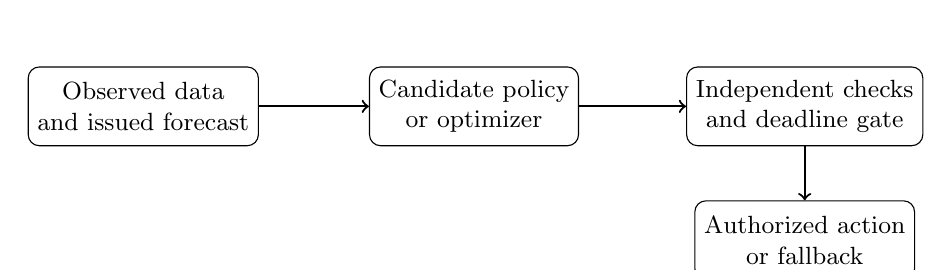
\begin{tikzpicture}[every node/.style={draw,rounded corners,align=center,font=\small,minimum height=1cm}]
\node (a) at (0,0) {Observed data\\and issued forecast};
\node (b) at (4.2,0) {Candidate policy\\or optimizer};
\node (c) at (8.4,0) {Independent checks\\and deadline gate};
\node (d) at (8.4,-1.7) {Authorized action\\or fallback};
\draw[->,thick] (a)--(b);\draw[->,thick] (b)--(c);\draw[->,thick] (c)--(d);
\end{tikzpicture}
\end{center}

\subsection{The trust chain}
A certificate proves something about an encoded instance and specification. The chain includes input identity, units, model construction, theorem or checking rule, arithmetic implementation, runtime environment, and physical actuation. Reducing the trusted code base can help, but it does not eliminate the need to validate sensors or model assumptions.

LP primal/dual witnesses can establish objective equality using exact arithmetic when rational data and witnesses are available. Floating-point solutions require justified reconstruction or interval bounds; rounding a dual vector can violate feasibility and invalidate a lower bound. For nonconvex OPF, a feasible point and a relaxation bound should be checked separately. For MILP, checking an incumbent is simpler than validating a global optimality claim; discrete proof artifacts and solver support differ.

Formal proofs of a controller's invariant can cover a bounded model and disturbance set. They do not establish that the real plant always stays within that set. Monitor envelope violations and make the fallback safe under the same timing and actuation assumptions.

\subsection{Deadlines and failure accounting}
Measure the complete path from observation availability to committed action, not just the optimizer's inner loop. Include parsing, preprocessing, data transfer, certificate generation, checking, and fallback selection. Report tail latency and missed deadlines alongside objective quality. A mean runtime below the sampling period is insufficient.

Treat timeout, infeasibility, numerical error, malformed input, and checker rejection as explicit outcomes. Score the resulting fallback trajectory, rather than dropping failed instances. A method can improve typical objective values while worsening service through rare failures. That tradeoff belongs in the main results.

\subsection{Independence must be designed}
Different implementations can share a model error; two kernels can check the same unintended theorem; two LLMs can share a reasoning pattern. Use separate formulations, dimensional checks, negative controls, known infeasible instances, and adversarial perturbations. Document shared dependencies. The VP/VNP audit is instructive because it distinguishes proof acceptance from statement correspondence and human understanding; the same distinctions apply to grid certificates.

\section{Reproducible preliminary experiments}
\label{sec:results}
\status{Executed locally on November 24, 2026. Exploratory, deliberately small tests; no preregistered statistical evaluation or field deployment.}

The package contains the complete Python implementation, unmodified public PGLib case and license, generated BESS inputs, every hourly schedule, all AC starts, solver settings, and machine-readable results. The runs used Python 3.12.9, NumPy 2.2.4, SciPy 1.18.0, and macOS 27.0.1 on ARM. BLAS and OpenMP thread environment variables were set to one. These settings do not establish deterministic wall-clock performance or a hard real-time guarantee.

\subsection{E01: small AC-OPF, a null improvement result}
The case is PGLib-OPF v23.07 \texttt{case3\_lmbd}, downloaded at repository commit
\texttt{dc6be4b2f85c} (full hash in the results file). It has three buses and three branches, 315\,MW active demand, and a 100\,MVA base. The implementation uses polar voltages, fixes one reference angle, and optimizes two active and three reactive generator outputs. It includes branch charging, active and reactive balances, generator bounds, voltage limits, both-end apparent-power limits, and angle-difference bounds. It is a single-period AC-OPF, not security-constrained dispatch.

SciPy SLSQP minimized the quadratic generation cost divided by 10,000 for scaling, with \texttt{ftol}$=10^{-10}$ and at most 1,000 iterations. The first start uses unit voltage magnitudes and zero angles; nine additional starts perturb those quantities with seed 20261124. The comparator is the first start against the best of all ten. Multistart consumes more computation; it is not an equal-budget algorithm comparison.

A separate branch-by-branch reconstruction checks the final balances rather than using the optimizer's Y-bus residual function. The acceptance thresholds are $10^{-5}$\,MVA for balances and thermal violations, $10^{-5}$ degrees for angle violations, and $10^{-7}$ in the encoded variable-bound units. The two implementations still share the case interpretation and branch equations; independence is partial.

\begin{table}[ht]
\centering\begin{tabular}{lr}
\toprule E01 measurement & Result\\\midrule
Accepted solver outcomes &10 of 10\\
Feasible cost range (\$/h) &5812.642974235398--5812.642974235489\\
Active network loss (MW, approximately) &3.073200\\
Largest balance residual (MVA) &$6.93\times10^{-12}$ or less\\
Largest reported thermal/angle/bound violation &0\\
Per-start elapsed time, observed (s) &0.0306--0.0351\\
Analytic lossless lower bound (\$/h) &5638.967948718\\
Feasible objective minus lower bound (\$/h) &173.675025517\\
Relative bound interval, using feasible cost &2.9879\%\\
\bottomrule
\end{tabular}
\caption{E01 results from the recorded run. Timing is an uncontrolled local observation.}
\end{table}

The additional starts produce no material objective improvement: the full cost spread is below $10^{-9}$ dollars per hour. The case's own documented objective of approximately \$5812.64/h is a useful sanity comparison, not an independently replayed global-optimality certificate.

\textbf{Derivation of the lower bound.} Positive branch resistance and zero real shunts imply generation at least equals active demand. The two active-generator cost functions are increasing and convex over their nonnegative domain. Dropping network and reactive constraints and allowing total generation to equal demand therefore enlarges the feasible set. With costs $a_1p_1^2+b_1p_1+a_2p_2^2+b_2p_2$ and $p_1+p_2=D$, the interior minimizer is
\[
 p_1=\frac{2a_2D+b_2-b_1}{2(a_1+a_2)},\qquad p_2=D-p_1.
\]
The code checks nonnegative resistances and that these values lie within generator active bounds. The supplied case has zero constant cost terms. Evaluating this relaxed dispatch yields the stated lower bound. It is a bound for this encoded case; it is not a general-purpose AC relaxation implementation.

The \$173.675 interval includes network and loss restrictions removed by the bound. It is not a measured pool of savings. No new solver, learned cut, VP/VNP-derived algorithm, contingency analysis, or proof of global AC optimality was implemented.

\subsection{E05: storage service, loss, and baseline sensitivity}
The synthetic system has a 100\,MW import cap, 50\,MW charge and discharge limits, 200\,MWh maximum energy, 40\,MWh reserve floor, 100\,MWh initial energy, and final energy at least 100\,MWh. Charge and discharge efficiencies are each 0.95. Import ramping is limited to 20\,MW per hour, starting from 80\,MW. Time steps are one hour over a 24-hour horizon.

The balances are
\begin{align}
 g_t+d_t-c_t+u_t&=\ell_t,\\
 e_{t+1}&=e_t+0.95c_t-d_t/0.95.
\end{align}
Here $g$ is import, $d$ discharge, $c$ charge, $u$ unserved load, and $\ell$ requested load. Nonnegative $u_t\le\ell_t$ makes inadequacy explicit. These are constructed profiles, not measured data-center traces:
\begin{itemize}
\item Flat: 80\,MW throughout.
\item Four-hour peak: sixteen hours at 80\,MW, four at 140\,MW, four at 80\,MW.
\item Eight-hour peak: twelve hours at 80\,MW, eight at 140\,MW, four at 80\,MW.
\item Alternating: twelve hours at 80\,MW, four alternating 140/80\,MW pairs, then four hours at 80\,MW.
\end{itemize}

Three policies use the same physical limits. The simple threshold policy recharges only to the initial 100\,MWh target and shaves imports above the cap. The forecast-aware threshold charges toward 200\,MWh whenever a future above-cap peak remains, then restores the initial target. The lookahead LP uses the complete deterministic profile and lexicographically minimizes total unserved energy, then charge-plus-discharge throughput. The LP relaxation permits simultaneous charging/discharging in principle; every returned schedule was checked to have no simultaneous operation. This observed property is not asserted for arbitrary modified inputs.

\begin{table}[ht]
\centering\begin{tabular}{lrrr}
\toprule Unserved energy (MWh) & Simple threshold & Forecast threshold & LP\\\midrule
Flat &0&0&0\\
Four-hour peak &103&8&8\\
Eight-hour peak &263&168&168\\
Alternating &48.85&0&0\\\bottomrule
\end{tabular}
\caption{The apparent LP advantage disappears against the stronger policy comparator.}
\label{tab:bess}
\end{table}

Relative to the simple threshold, the LP serves an additional 95\,MWh in each continuous-peak case and 48.85\,MWh in the alternating case. Relative to the forecast-aware rule, it adds zero service on all four cases. The two stronger policies also have matching aggregate imports, throughput, losses, and terminal energy within floating-point tolerance. This ablation was added after the first comparison; the study is exploratory.

The improvement against the weaker comparator has an energy cost. In the four-hour peak case, storage conversion losses rise from 6.157895 to 16.421053\,MWh, and grid imports rise from 2063.157895 to 2168.421053\,MWh. Serving more demand is not synonymous with reducing energy losses. In the alternating case, losses rise from 12.007895 to 17.285319\,MWh while unserved load falls to zero. The package records each balance and schedule so these conclusions can be checked directly.

\textbf{A physical lower bound is attained.} The continuous four-hour deficit above the import cap is $4\cdot40=160$\,MWh. The most that a fully charged device can deliver above its reserve floor is $0.95(200-40)=152$\,MWh. Equation~\eqref{eq:storagebound} therefore requires at least 8\,MWh unserved; both stronger policies attain it. The eight-hour deficit is 320\,MWh, leaving at least 168\,MWh unserved. Zero is the universal lower bound for the other two profiles, and it is attained. This establishes minimal unserved energy for these four specified profiles under the model; it does not establish a general policy theorem.

All twelve schedules passed energy, power-balance, bounds, ramp, terminal, and nonsimultaneity checks. The largest recorded numerical violation is below $10^{-12}$. The two-stage LP took approximately 0.0028--0.0109 seconds per profile in the recorded run. This is not a closed-loop MPC evaluation, a forecast-error test, a frequency or voltage study, an aging model, a revenue backtest, or a reliability accreditation study.

\subsection{E04: a small exact certificate and negative controls}
Consider the rational LP
\[
 \min 20x+50y\quad\text{subject to }x+y=100,\quad0\le x\le60,\quad y\ge0.
\]
The witness $(x,y)=(60,40)$ has objective 3200. The dual witness $(\lambda,\mu)=(50,30)$ obeys $\mu\ge0$, $\lambda-\mu\le20$, and $\lambda\le50$, with lower bound
\[
 100\lambda-60\mu=3200.
\]
Weak duality and equality certify this toy optimum under the stated rational model. The checker uses Python's \texttt{Fraction}; it accepts the witness and rejects four alterations: a capacity breach, a changed equality multiplier, a changed bound multiplier, and a demand-balance breach.

This is an exact-arithmetic demonstration, not a verified implementation of a checker, not a Lean proof, and not an AC-OPF or SCUC certificate. Four rejected mutations illustrate controls; they do not prove that every malformed certificate would be rejected. Its purpose is to demonstrate the candidate/witness/checker separation at a scale where every step is inspectable.

\subsection{VP-review checks reproduced}
The supplied review's three Python scripts were copied with their required pinned transition-rule source, license, and notice. Their outputs are included separately from the grid benchmark results. Exact fraction checks reproduce the flat-branch numerical margin and the mixed-cut example; pointer enumeration exhausts its four finite examples; the cut script checks 16 expanded weighted terms and 15 resource cases. This reproduces selected diagnostics, not the paper's universal lemmas. The previous review's focused Lean outcomes remain \emph{reported historical executions}; no Lean compilation was performed for this edition.

\subsection{What was not run}
E02 (unit commitment/SCUC), E03 (converter MPC), and E06 (fleet economics and adequacy) were not executed. No ARPA-E GO full challenge, large PGLib suite, hardware-in-the-loop study, field pilot, or complete VP/VNP proof replay was run. Their protocols below are proposed work. Tables of expected outcomes or invented performance numbers are deliberately absent.

\section{Uncertainty, statistical validity, and falsification}
\label{sec:uncertainty}
\subsection{What the preliminary panel can support}
The four battery profiles were constructed to expose mechanisms, not sampled from an operating distribution. Ten AC starting points are not ten independent network instances. A confidence interval around their mean would not quantify population performance. This edition consequently reports exact instance-level results and no fleet extrapolation, significance test, or probability of commercial success.

For a future chronological study, use paired realizations: each baseline and candidate sees the same load, weather, outages, and forecast issues. Define $\Delta_i=Q_{1i}-Q_{0i}$ on held-out blocks. An estimate $\hat\Delta=\sum_iw_i\Delta_i$ needs weights representing the target population. If difficult hours are oversampled, inverse selection weights or a separately reported stress panel are required.

Temporal correlation makes an hour-by-hour independent bootstrap inappropriate. Use weather-year or operational-block resampling aligned with the dependence structure. Report sensitivity to block length and to exclusion of individual extreme events. Training, tuning, and evaluation periods must be separated; topology and outage changes should appear in the holdout, not merely random rows from the same day.

\subsection{Failure probability and rare events}
With zero failures in $n$ genuinely independent Bernoulli trials under a fixed failure definition, a one-sided $(1-\alpha)$ upper confidence bound is
\[
 p_{\max}=1-\alpha^{1/n}.
\]
At $\alpha=0.05$, roughly 2,995 independent trials are needed before this bound falls below $0.001$. This conditional calculation is not an assurance claim for correlated grid operations. Common-mode failures, distribution shifts, and unobserved extreme events can invalidate the model. In such cases, scenario testing and formal envelope arguments complement rather than replace empirical evidence.

A noninferiority test for reliability must prespecify an acceptable margin in the actual risk metric. A positive mean cost benefit cannot compensate for an unapproved increase in critical-load interruption. If reliability is a hard constraint, reject candidates violating it rather than subtracting an arbitrary penalty after seeing the result.

\subsection{Risk-sensitive objectives}
A proposed risk-sensitive cost criterion could use
\[
 \min_\pi \E[C_\pi]+\lambda\operatorname{CVaR}_\beta(C_\pi),
 \qquad
 \operatorname{CVaR}_\beta(C)=
 \min_\eta\left\{\eta+\frac{\E[(C-\eta)_+]}{1-\beta}\right\}.
\]
The confidence level $\beta$, weight $\lambda$, and scenario model require a stakeholder decision. They are not parameters to tune retrospectively until the candidate appears favorable. A risk-sensitive objective does not eliminate the need for explicit physical safety constraints.

Uncertainty about battery efficiency, available energy, thermal ratings, or demand forecast can be handled through scenario, robust, or distributionally robust models. The ambiguity set and coverage claim must be justified by data or engineering limits. Enlarging the uncertainty set can reduce service; that conservatism has a measurable cost but may be necessary to honor the contract.

\subsection{Selection, survivorship, and hidden budgets}
Report every eligible case, including failures and timeouts. Maintain a record of rejected ideas and tuning trials so development compute is not hidden. A learned policy selected from thousands of searches should not be compared with a single untuned baseline and described as cheaper without accounting for amortization.

A failure to retrieve a source is a coverage gap, not evidence that the claim lacks support everywhere. Similarly, a failed numerical solve is not proof of physical infeasibility. Preserve the distinction between model infeasibility, algorithm failure, data error, and missing evidence.

\section{A falsifiable research program}
\label{sec:program}
\subsection{E01 extension: AC-OPF and security-constrained operations}
Use the PGLib normal and stressed families, then a separate security-constrained challenge with documented contingency requirements. Pin the data and formulation before tuning. Compare strong nonlinear solvers, warm starts, and established convex or moment relaxations. Record feasible cost, best bound, balance and limit residuals, failed solves, memory, and complete latency.

A proposed AI-guided ordering, cut, or decomposition must have an ablation that removes only that component. Include a shuffled or random-order control when applicable. Freeze equal compute and tuning budgets. Reject the claimed benefit if it disappears after feasibility repair, independent validation, or comparison with a tuned conventional method. A tiny benchmark result does not advance this gate.

\subsection{E02: commitment under realistic timing}
Begin with PGLib-UC to compare formulations and incumbent quality. Add a documented network and contingency formulation before using the label SCUC. Include minimum up/down histories, startup categories, ramp limits, reserves, outages, and sub-hourly requirements where relevant. Compare a strong MILP baseline with the candidate under identical time limits.

Use a rolling simulation with issued forecasts and realized dispatch. Preserve commitment decisions between solves and record emergency actions. Evaluate starts, fuel, unserved energy, reserve deficiencies, and deadline failures. Test warm-start quality separately from a changed forecast or objective. The principal falsifier is that objective improvement vanishes when a stronger formulation or operationally feasible chronology is used.

\subsection{E03: converter MPC and implementation}
Choose a documented converter and filter model, sampling rate, processor, numerical representation, and disturbance envelope. Compare existing PI or other deployed control, a well-tuned MPC baseline, and the candidate. Test parameter drift, saturation, sensor noise, communication delay, and weak-grid conditions. Measure electrical losses, tracking quality, stability margin, and end-to-end worst-case timing.

Advance from numerical simulation to controller hardware and then power hardware only with an independently reviewed safety case. A faster optimization subroutine is insufficient if sensing and actuation dominate latency. The candidate is falsified for the target envelope by an unacceptable stability, current, voltage, thermal, or deadline failure.

\subsection{E04 extension: certificates that matter to a decision}
Choose one supported model and certificate type. Define the exact theorem and data encoding. Separate discovery from checking; include invalid instances, altered units, stale inputs, and malformed witnesses. For numerical bounds, use exact reconstruction or rigorous enclosures where needed.

Measure acceptance coverage, rejection causes, certificate size, check time, and the operational action enabled. A successful proof that changes no admissible action may still be valuable research, but it has no demonstrated dispatch value. Compare a small trusted checker with an independent calculation, and document the remaining trusted components.

\subsection{E05 extension: large-load BESS with imperfect forecasts}
Acquire a permitted load trace and its forecast history, not only a plotted demand curve. Specify UPS reserve, cycling cost, thermal derating, contractual service, and utility import/ramp constraints. Include the simple forecast-aware threshold from this edition as a mandatory comparator.

Run rolling horizons with forecast errors, correlated charging restrictions, long deficits, and battery outages. Compare same-hardware policies first; then vary hardware in a separate factorial experiment. Record useful service, unserved MWh, peak shortfall, losses, cycling, reserve violations, and terminal energy. The candidate's computational value is falsified if the simple rule matches it after realistic errors and costs.

\subsection{E06: portfolio economics and capacity}
Only after credible operational gains exist should the study estimate population value. Build a weighted instance population with nodal and seasonal coverage. Reconcile energy and monetary ledgers, compute implementation costs, and run chronological adequacy with correlated weather and outages.

Estimate risk-equivalent load-carrying capability separately from annual energy. Reoptimize affected network states; do not multiply a local shadow price by an arbitrarily large change. Commercial claims require a defined beneficiary, contracting rights, market eligibility, and costs. The upper-bound test can terminate the program if even its optimistic physically feasible benefit is below deployment cost.

\subsection{Stage gates}
\begin{longtable}{P{.17\linewidth}P{.44\linewidth}P{.30\linewidth}}
\toprule Gate & Evidence required & Current status\\\midrule\endhead
G0: identity & Recovered inputs, source lineage, explicit unresolved files and versions & Partial: Napkin preserved; v0.1 full files unavailable; Atlas unresolved.\\
G1: executable model & Reproducible inputs, numerical checks, negative controls & Passed for small stated models only.\\
G2: comparative benefit & Strong baselines, equal budgets, held-out cases, reliability contract & Not passed. Current ablations show null optimization-specific effects.\\
G3: operational assurance & Deadline, fallback, uncertainty and dynamics tests & Not run.\\
G4: field and economic value & Authorized pilot, independent measurement, cost and attribution audit & Not run.\\
\bottomrule
\end{longtable}
These gates distinguish a completed document from a completed research program. This edition delivers the document and a preliminary panel; it does not claim G2--G4.

\section{Skeptical objections and decisive responses}
\label{sec:skeptics}
\begin{longtable}{P{.27\linewidth}P{.38\linewidth}P{.26\linewidth}}
\toprule Objection & Assessment & Evidence that would resolve it\\\midrule\endhead
This is existing optimization under a new name. & Much of the technical machinery is existing work. The proposed contribution is attribution, assurance, and comparable service accounting. Novel algorithmic claims are not made. & Demonstrate a new validated mechanism or a materially useful measurement framework against prior work.\\
The VP/VNP theorem is a distraction. & It supplies no grid speedup. Its transferable lesson is a candidate/checker workflow and careful statement scope. & An explicit reduction or implemented method with measured incremental benefit.\\
The proof has not received broad human validation. & Primary artifacts and reported machine checks exist; complete independent mathematical review is not established here. & Reconstructed dependencies, full replay at pins, and independent expert review.\\
The Napkin double counts money and energy. & The additive recovery estimate is excluded. Ledger boundaries and counterfactuals are now explicit. & A reconciled chronological system and cash-flow study.\\
Operators already use strong solvers. & This is a central baseline requirement. Comparing with an artificially weak method inflates apparent value. & Current formulations, hardware, settings, and actual operational constraints.\\
The battery gain is just better planning. & On this panel a simple forecast-aware rule matches the LP. An optimizer-specific gain is not demonstrated. & Held-out imperfect-forecast cases where a candidate beats that rule net of costs.\\
The OPF gap is an artifact of a weak bound. & The analytic bound removes network restrictions. It measures uncertainty, not actual recoverable savings. & Stronger valid lower bounds and independently feasible candidate improvements.\\
Formal verification proves the model, not the grid. & Agreed in scope: input semantics, omitted physics, and plant/model mismatch remain obligations. & An end-to-end assurance argument plus field and envelope evidence.\\
More service may increase energy consumption. & It does in the constructed BESS cases. Report useful service and losses separately. & A service-equivalent comparison if energy efficiency is the objective.\\
Annual TWh cannot supply scarcity-hour MW. & Average power is not capacity credit. & Chronological risk-equivalence and deliverability assessment.\\
The economics omit deployment costs. & No commercial estimate is admitted in this edition. & Integration, compute, validation, degradation, maintenance, and contractual cash flows.\\
The Library review is incomplete. & The bounded coverage is disclosed; inventory is not full reading. & Verified Atlas/native Library routing and resolution of missing source files.\\
\bottomrule
\end{longtable}

\section{Source governance, coverage, and limitations}
\label{sec:sources}
\subsection{What was inventoried and searched}
The local \texttt{Research \& Knowledge/\_GOVERNANCE/prompts/START\_HERE.md} and its routing, governance, authority, freshness, and risk configurations were read. Relevant routes included Grid \& Energy and AI research. The local traversal covered seven domain roots: Energy\_Grid; Mathematics; Computer\_Science; AI\_ML; Electrical\_Engineering\_and\_Systems; Power Systems Study Review Series; and Energy \& UEVF Projects within the internal collaboration material.

The inventory contains 1,451 files and marks 67 filename candidates. A first-two-page screen covers 293 subject PDFs and identifies 24 keyword matches. Thirteen selected PDFs were fully text-extracted, but extraction is not equivalent to critical reading of every page. The 716-page internal compilation, for example, is listed as a compilation and is not treated as 716 pages of independent reviewed evidence. Selected claim-bearing passages and publication identities were examined.

Drive queries included CRGC, START\_HERE, Atlas, computational load, BESS ramp, Grid \& Energy, Mathematics, and formal verification, with bounded result sets. Three relevant documents were fetched: the internal large-load synthesis, the LLM self-verification paper, and the grid-forming BESS paper. Local and Drive duplicates are one evidence lineage. Exact-name searches did not recover CRGC v0.1 or a relevant Atlas.

A prior folder registry is a routing hint, not a current native-Library inventory. The native Library's complete contents and an authoritative Atlas were not verified. The paper therefore does not claim exhaustive review of the user's entire Library or Drive. The companion inventories preserve search scope, source roles, retrieval levels, and remaining gaps.

\subsection{Primary, independent, and internal evidence}
Primary technical papers are used for their own theorem or experiment claims. Official reports are used for their stated measurements or projections, retaining caveats and source dependence. A DOE summary of another organization's estimate does not create independent corroboration. Public commentary on VP/VNP is attributed as an audit report rather than promoted to consensus.

Internal manuscripts, the Napkin, and the six-pass VP review are identifiable internal research. They can contribute hypotheses, definitions, and traceable checks. They cannot independently corroborate their own market-size or scientific-efficacy claims. This study's benchmark outputs form another explicitly limited evidence group.

The source inventory records exact links and available hashes. It does not redistribute the entire private Library, Drive downloads, or third-party PDFs. The included public case retains its license. The source inventories contain private paths and should remain confidential with this packet.

\subsection{Preservation and unavailable inputs}
The Napkin copy has SHA-256
\begin{center}\small\texttt{0287ae357176cbc5235459a9e7f1c3739981f5e4e0abd8477730f5c67d995be3}.\end{center}
The referenced chat contains download links for \texttt{CRGC\_Whitepaper\_v0.1.tex} and its PDF, but those files were not available through the retrieved chat or local/Drive searches. Its inline LaTeX terminates mid-document. That exact excerpt is saved with a \texttt{.tex.txt} suffix and an explicit incomplete-source notice. No reconstructed file is passed off as the original.

The supplied VP review remains unedited. Its source manifest, pass records, selected proof interfaces, and checks were read; only copies needed for reproducible finite diagnostics are included in this packet. The full Lean project was not rebuilt. No Library or Drive originals were moved or edited, and no artifact was publicly uploaded or shared.

\subsection{Material limitations}
This is a synthesis with small executed demonstrations, not an independently refereed proof audit, an exhaustive systematic review, or an operational grid study. The experiments omit security contingencies, forecast uncertainty, transient dynamics, realistic markets, field reliability, and deployment costs. The AC case is extremely small; the battery profiles were constructed; the certificate is a toy rational LP.

Literature coverage varies from full-document extraction and selected passage review to abstract and repository documentation review. Each source's coverage is recorded rather than implied by its presence in a bibliography. Fast-moving November 2026 mathematical claims may be revised after this evidence cutoff. Results should be updated by version, not overwritten without provenance.

\section{Conclusions and the next decision}
The defensible CRGC thesis is that operationally admissible decisions can be compared for useful service, resource cost, risk, and computational expense under a fixed contract. This paper establishes a way to make that comparison auditable. It does not establish a national pool of recoverable energy.

The executed panel supplies three useful findings. More AC starting points did not materially improve the chosen case. Better preparation for known peaks improved battery service relative to a limited policy, but a simple forecast-aware rule captured all the measured advantage. Exact certificates can be separated from candidate generation in a small inspectable example. These findings favor stronger baselines and precise contracts before expensive deployment claims.

The VP/VNP releases deserve continued mathematical examination, but CRGC does not depend on their validity. The immediate research decision is to select one operational bottleneck with permitted data and a credible comparator, then run the corresponding held-out protocol. If no net benefit survives that test, the associated CRGC claim should be retired. If a benefit survives, its magnitude remains local until a separate population and reliability study supports broader use.

\appendix
\section{Reproduction and artifact map}
The LaTeX source contains its own bibliography and diagram and compiles without external figures or bibliography files. A Tectonic build was used for the supplied PDF. The accompanying README gives commands, dependency versions, and output meanings.

\begin{longtable}{P{.42\linewidth}P{.49\linewidth}}
\toprule Artifact & Purpose\\\midrule\endhead
\texttt{CRGC\_Whitepaper\_v0.2.tex/.pdf} & Standalone source and compiled master document.\\
\texttt{source\_inventory\_local.csv} & Bounded local metadata inventory; not a claim that every file was read.\\
\texttt{source\_inventory\_read.json} & PDF extraction record, hashes, and page counts.\\
\texttt{library\_abstract\_screen.json} & First-two-page screening record.\\
\texttt{sources.csv}, \texttt{sources.json} & Curated references, lineage, anchors, and retrieval scope.\\
\texttt{claim\_evidence\_map.csv} & Claims, evidence status, limitations, and experiment links.\\
\texttt{gaps\_and\_limitations.md} & Unresolved inputs and validation gates.\\
\texttt{reproducibility/} & Code, public case, synthetic inputs, schedules, results, and finite VP-review diagnostics.\\
\texttt{preserved/} & Unchanged Napkin and separately labeled incomplete v0.1 excerpt.\\
\texttt{quality\_report.json} & Technical checks and explicit unresolved completeness gates.\\
\bottomrule
\end{longtable}
Re-running the benchmark script overwrites its local output JSON/CSV files. Copy the reproducibility folder first to preserve the delivered run. Solver timing may vary. Neither successful execution nor a matching result substitutes for independent review of the model and validation logic.

\section{Compact claim register}
\begingroup\small
\begin{longtable}{P{.10\linewidth}P{.46\linewidth}P{.35\linewidth}}
\toprule ID & Claim & Disposition\\\midrule\endhead
C01 & CRGC is a baseline-relative, contract-specific outcome. & Definition proposed here.\\
C02 & November releases claim VP/VNP separation over every field. & Primary statements verified; full proofs not replayed here.\\
C03 & The separation supplies an AC-OPF or SCUC solver. & Unsupported; excluded.\\
C04 & Ten percent of the Napkin pools is recoverable. & Unvalidated scenario; excluded from findings.\\
C05 & The Napkin arithmetic yields 8.26/46.87 TWh. & Derived from its inputs; no causal validation.\\
C06 & 46.87 TWh implies 5.35 GW firm capacity. & Average-power arithmetic only; firm-capacity claim excluded.\\
C07 & MISO's ratings opportunity is realized solver savings. & Unsupported attribution; source reports estimated ratings opportunity.\\
C08 & A certified optimization gap equals realized savings. & Unsupported; it can bound remaining same-model improvement.\\
C09 & Multistart improves the tested AC case materially. & Not observed.\\
C10 & LP BESS planning beats a forecast threshold on this panel. & Not observed; service and aggregate energy match.\\
C11 & Serving more load must reduce losses. & Contradicted by the constructed BESS comparison.\\
C12 & Toy rational witness passes; four mutants fail. & Executed exact-arithmetic check; limited scope.\\
C13 & Full Library and Atlas context was reviewed. & Not established; bounded coverage disclosed.\\
C14 & Selected VP-review finite diagnostics reproduce. & Executed; not a general proof or full Lean replay.\\
C15 & Commercial value or accredited MW is established. & Not established; E06 unrun.\\
\bottomrule
\end{longtable}
\endgroup
\clearpage
\phantomsection\addcontentsline{toc}{section}{References}
\begin{thebibliography}{99}
\bibitem{anthropic} Claude (Anthropic). \emph{VP $\ne$ VNP Over Every Field}. 2026-11-23. \href{https://github.com/anthropics/formal-math/blob/11b6c7e3c927df2658f513b6b68ea7f8929c62c5/vp-vnp/paper.pdf}{Primary source}. 70-page paper: pp.1-7; theorem statements; Appendix Q via supplied review.

\bibitem{anthropicstatement} Anthropic. \emph{Statement.lean: arithmetic circuit definitions and separation statements}. 2026-11-23. \href{https://github.com/anthropics/formal-math/blob/11b6c7e3c927df2658f513b6b68ea7f8929c62c5/vp-vnp/Statement.lean}{Primary source}. Computes; MainTheorem; Approximates; MainTheoremApprox; SeparationClosure.

\bibitem{anthropicrepo} Anthropic. \emph{Formal-math VP/VNP release README}. 2026-11-23. \href{https://github.com/anthropics/formal-math/blob/main/vp-vnp/README.md}{Primary source}. Authorship notice; checking workflow; Challenge versus Solution.

\bibitem{openai} OpenAI. \emph{VP and VNP are different}. 2026-11-23. \href{https://github.com/openai/math/blob/main/preprints/VP-and-VNP-are-different-November-23-2026/paper.pdf}{Primary source}. Theorem 1.1; Corollary 1.2; contents and introduction pp.1-3; README.

\bibitem{toledo} Carlos Toledo. \emph{The VP $\ne$ VNP claim, checked in the open}. 2026-11-24 03:15 UTC snapshot. \href{https://carlostoledo.co/vp-vnp/}{Primary source}. Verdict; 18/23 rows; limits; constant; pinned target and change log.

\bibitem{internalvp} User-supplied internal research review. \emph{VP-VNP Chat Handoff, Edition 3, and passes 1-6}. 2026-11-24. Internal source; see companion inventory. README; source-lock; six passes; checks; selected Alternative.lean interfaces.

\bibitem{go} Pacific Northwest National Laboratory. \emph{Supporting ARPA-E Power Grid Optimization: Final Scientific/Technical Report, PNNL-36158}. 2024-06-30. \href{https://www.osti.gov/servlets/purl/2404530}{Primary source}. PDF pp.4-5, executive summary and challenge description.

\bibitem{pglib} Sogol Babaeinejadsarookolaee et al.. \emph{The Power Grid Library for Benchmarking AC Optimal Power Flow Algorithms}. 2019; arXiv v2 2021. \href{https://arxiv.org/abs/1908.02788}{Primary source}. Abstract; repository README; v23.07 case3\_lmbd.

\bibitem{pglibuc} Power Grid Library contributors. \emph{PGLib-UC benchmark library README}. v19.08. \href{https://github.com/power-grid-lib/pglib-uc/blob/master/README.md}{Primary source}. Problem formulation: global demand and reserve; unit constraints.

\bibitem{low1} Steven H. Low. \emph{Convex Relaxation of Optimal Power Flow, Part I: Formulations and Equivalence}. 2014. \href{https://arxiv.org/abs/1405.0766}{Primary source}. Abstract and formulations overview; DOI 10.1109/TCNS.2014.2309732.

\bibitem{low2} Steven H. Low. \emph{Convex Relaxation of Optimal Power Flow, Part II: Exactness}. 2014. \href{https://arxiv.org/abs/1405.0814}{Primary source}. Sufficient conditions; DOI 10.1109/TCNS.2014.2323634.

\bibitem{moment} Daniel K. Molzahn, Cedric Josz, Ian A. Hiskens, Patrick Panciatici. \emph{Computational Analysis of Sparsity-Exploiting Moment Relaxations of the OPF Problem}. 2016. \href{https://arxiv.org/abs/1603.05188}{Primary source}. Abstract and method scope.

\bibitem{hardness} Daniel Bienstock, Abhinav Verma. \emph{Strong NP-hardness of AC power flows feasibility}. 2015; v2 2019. \href{https://arxiv.org/abs/1512.07315}{Primary source}. General-network feasibility result.

\bibitem{uc} Bernard Knueven, Jim Ostrowski, Jean-Paul Watson. \emph{On Mixed-Integer Programming Formulations for the Unit Commitment Problem}. 2020. \href{https://optimization-online.org/wp-content/uploads/2018/11/6930.pdf}{Primary source}. Abstract; IJOC 32(4), 857-876; DOI 10.1287/ijoc.2019.0944.

\bibitem{round} Shaked Regev, Eve Tsybina, Slaven Peles. \emph{Fast Relax-and-Round Unit Commitment with Sub-hourly Mechanical and Ramp Constraints}. 2026; arXiv v4. \href{https://arxiv.org/abs/2602.03977}{Primary source}. Abstract; local older 8-page edition versus live v4.

\bibitem{experiment} Jose Daniel Lara, Jonathan T. Lee, Duncan Callaway, Bri-Mathias Hodge. \emph{Computational Experiment Design for Operations Model Simulation}. 2020. \href{https://arxiv.org/abs/2004.11517}{Primary source}. Experiment-design framework; DOI 10.1016/j.epsr.2020.106680.

\bibitem{mpc} Min Jeong, Manuel Schoen, Jurgen Biela. \emph{When FPGAs Meet ADMM with High-level Synthesis (HLS): A Real-time Implementation of Long-horizon MPC for Power Electronic Systems}. 2023. \href{https://www.research-collection.ethz.ch/server/api/core/bitstreams/63c29e96-9bf9-4714-a4e3-cd4dc4fb8bde/content}{Primary source}. Abstract; exemplary inverter implementation.

\bibitem{mpc2} Min Jeong, Simon Fuchs, Jurgen Biela. \emph{When FPGAs Meet Regionless Explicit MPC: An Implementation of Long-horizon Linear MPC for Power Electronic Systems}. date not independently resolved. \href{https://www.research-collection.ethz.ch/server/api/core/bitstreams/c293d2db-8673-4ddc-ba71-1dd3afa0cff2/content}{Primary source}. Primary repository indexed abstract/title.

\bibitem{mpcdamp} Min Jeong, Tino Gfrorer, Jurgen Biela. \emph{Extending Stable Parameter Range of LCL-filters for Grid-Connected Converters by Inherent Damping of MPC}. 2022. \href{https://www.research-collection.ethz.ch/bitstream/handle/20.500.11850/564410/3/LCL_filter_MPC_COMPEL2022_final_submission.pdf}{Primary source}. Primary paper abstract and scope.

\bibitem{complexity} Shamisa Shoja, Daniel Arnstrom, Daniel Axehill. \emph{Parallel Domain-Decomposition Algorithms for Complexity Certification of Branch-and-Bound Algorithms for Mixed-Integer Linear and Quadratic Programming}. 2025. \href{https://arxiv.org/abs/2503.16411}{Primary source}. Local first two pages: abstract and introduction.

\bibitem{leanpep} Xinyuan Guo, Andersen Ang. \emph{Lean-PEP: Performance-Estimation Certificates to Formally Verified Algorithmic Bounds}. 2026-11-13. \href{https://arxiv.org/abs/2611.17618}{Primary source}. Abstract; supported PG/GD interface and exact certificate scope.

\bibitem{selfverify} Kaya Stechly, Karthik Valmeekam, Subbarao Kambhampati. \emph{On the Self-Verification Limitations of Large Language Models on Reasoning and Planning Tasks}. 2024. \href{https://arxiv.org/abs/2402.08115}{Primary source}. Abstract and task/model scope; Drive file 1Uxq6Y4swzGuoWxKUuq-suNUmp\_Yp5asJ.

\bibitem{gridagent} Yan Zhang, Ahmad Mohammad Saber, Amr Youssef, Deepa Kundur. \emph{Grid-Agent: An LLM-Powered Multi-Agent System for Power Grid Control}. 2025; arXiv v2. \href{https://arxiv.org/abs/2508.05702}{Primary source}. Local first two pages: abstract and introduction.

\bibitem{gridcopilot} Sarthak Chaturvedi, Sichen Jin, Shrirang Abhyankar, Travis Thurber, Kostas Oikonomou, Nathalie Voisin. \emph{Grid CoPilot: A Large Language Model (LLM) Based Framework for Transforming Long-Term Planning Analyses}. 2025-04-17. \href{https://www.preprints.org/manuscript/202504.1464}{Primary source}. First two pages; DOI 10.20944/preprints202504.1464.v1.

\bibitem{nerc} North American Electric Reliability Corporation. \emph{Characteristics and Risks of Emerging Large Loads}. 2025-07. \href{https://www.nerc.com/globalassets/who-we-are/standing-committees/rstc/whitepaper-characteristics-and-risks-of-emerging-large-loads.pdf}{Primary source}. Executive scope and risks; local filename misattributes publisher as NREL.

\bibitem{lbnl} Sarah Josephine Smith et al.. \emph{United States Data Center Energy Usage Report: 2025 Update}. 2026-06. \href{https://bies.lbl.gov/publications/united-states-data-center-energy-2025}{Primary source}. Official abstract: reference case 649 TWh in 2030; uncertainty scenarios.

\bibitem{gfm} Yousef Abudyak, Mohsen Alizadeh, Wei Sun. \emph{Mitigating Data Centers Load Risks and Enabling Grid Support Functions through Grid-Forming Control}. 2026. \href{https://arxiv.org/abs/2602.01013}{Primary source}. Abstract; simulation section; conclusion; Drive file 1zkzUv5K-1RNAvWlRs97rFtHafnoPbNh5.

\bibitem{split} Sheng Yin et al.. \emph{Price Aware Power Split Control in Heterogeneous Battery Storage Systems}. 2025-07-01. \href{https://arxiv.org/abs/2507.00628}{Primary source}. Abstract; local arXiv v1.

\bibitem{miso} Potomac Economics. \emph{2025 State of the Market Report for the MISO Electricity Markets}. 2026-06. \href{https://www.potomaceconomics.com/wp-content/uploads/2026/07/2025-State-of-the-Market-Report.pdf}{Primary source}. Printed p.68 / PDF p.94, Table 11 and footnote 24; congestion discussion.

\bibitem{doe} U.S. Department of Energy. \emph{National Transmission Needs Study: Draft}. 2026-07. \href{https://www.energy.gov/documents/national-transmission-needs-study-draft-july-2026}{Primary source}. Printed pp.37-38 and 47; congestion estimates and cited provenance.

\bibitem{elcc} Qian Zhang, Feng Zhao, Gord Stephen, Chanan Singh, Le Xie. \emph{A Gradient-Based Capacity Accreditation Framework in Resource Adequacy: Formulation, Computation, and Practical Implications}. 2026. \href{https://arxiv.org/abs/2601.22087}{Primary source}. Abstract and introduction, local p.1; regularity and marginal interpretation.

\bibitem{internaldls} Justin Candler / Nous Enterprises LLC. \emph{Large Loads, Inverter-Based Resources, and the New Grid Bottleneck}. 2026-03-26. Internal source; see companion inventory. PDF pp.10-13; assumptions and dependable-service vocabulary.

\bibitem{internalcompute} Justin Candler / Nous Enterprises LLC. \emph{Compute-ASCDE-SMR: A Reliability-Complete Valuation and Planning Interface for Nuclear-Coupled AI Campuses}. 2026-01-15 title date. Internal source; see companion inventory. Abstract and framing; header also says January 14.

\bibitem{napkin} User-supplied internal document. \emph{The Billion-Dollar Napkin}. undated copy supplied. Internal source; see companion inventory. Six-page original; pool arithmetic and value hypotheses.

\bibitem{v01} Referenced ChatGPT conversation. \emph{CRGC v0.1 incomplete inline LaTeX excerpt}. retrieved 2026-11-24. Internal source; see companion inventory. Conversation 6b05f106-044c-83ea-838c-39265ec16ff6.

\end{thebibliography}
\end{document}
